\documentclass{article}
\usepackage{graphicx} % Required for inserting images
\usepackage{kotex}
\usepackage{amsmath}
\usepackage{mathtools}
\usepackage{amsthm}
\usepackage[margin=2cm,nonhead]{geometry}
\usepackage{setspace}
\usepackage{abstract}
\usepackage{authblk}
\usepackage{multicol,layout,epsf,verbatim,array,tabularx,graphicx,kotex,amssymb,amsmath,setspace}
\usepackage{enumerate}
\usepackage{tikz}
\usetikzlibrary{
  hobby,
  intersections,
  spath3,
  decorations.markings,
  arrows.meta,
}

\newcommand{\czero}{
  \tikz[baseline=-0.6ex, scale=0.7]{
    \path (0,0) coordinate (base);
    \draw[line width=0.7pt] (0,0.4) .. controls (0.3,0.3) and (0.3,-0.3) .. (0,-0.4);
    \draw[line width=0.7pt] (0.8,0.4) .. controls (0.5,0.3) and (0.5,-0.3) .. (0.8,-0.4);
  }
}
\newcommand{\cinf}{
  \tikz[baseline=1.2ex, scale=0.7]{
    \path (0,0) coordinate (base);
    \draw[line width=0.7pt] (0.4, 0) .. controls (0.2, 0.3) and (-0.2, 0.3) .. (-0.4, 0);
    \draw[line width=0.7pt] (0.4, 0.8) .. controls (0.2, 0.5) and (-0.2, 0.5) .. (-0.4, 0.8);
  }
}

\newcommand{\Xslashfront}{
  \tikz[baseline=-0.6ex, scale=0.28]{
    \draw[line width=0.7pt] (-1,1) -- (1,-1);
    \draw[line width=4.0pt, white] (-0.5,-0.5) -- (0.5, 0.5);
    \draw[line width=0.7pt] (-1,-1) -- (1,1);
  }
}

\newcommand{\Xslashback}{
  \tikz[baseline=-0.6ex, scale=0.28]{
    \draw[line width=0.7pt] (-1,-1) -- (1,1);
    \draw[line width=4.0pt, white] (-0.5,0.5) -- (0.5,-0.5);
    \draw[line width=0.7pt] (-1,1) -- (1,-1);
  }
}

\onehalfspacing

\newcommand{\rarrow}{\rightarrow}
\newcommand{\larrow}{\leftarrow}

\newtheorem{thm}{Theorem}
\theoremstyle{definition}
\newtheorem{defn}[thm]{Definition}
\theoremstyle{theorem}
\newtheorem{theorem}{Theorem}
\theoremstyle{proposition}
\newtheorem{prop}{Proposition}
\theoremstyle{corollary}
\newtheorem*{corol}{Corollary}

\renewcommand\Affilfont{\small}

\title{R\&E 과제명 (영문)}
\author[1]{조은찬\thanks{email}}
\author[1]{Jeongwon Shin\thanks{io25jellyfish@gmail.com}}
\author[1]{서보연\thanks{이메일}}
\author[1]{최민호\thanks{이메일}}
\author[2]{김훈\thanks{이메일}}
\author[3]{진교택\thanks{이메일}}
\author[4]{이재원\thanks{이메일}}
\affil[1]{Researcher, Korea Scinece Academy of KAIST}
\affil[2]{Supervisor, Department of Mechanical Engineering, \LaTeX\ University}
\affil[3]{Co-Supervisor, Department of Computer Science, \LaTeX\ University}
\affil[4]{Assistant, Department of Computer Science, \LaTeX\ University}


\renewcommand\Authands{ and }

\date{\vspace{-5ex}}

\begin{document}

\maketitle

\renewenvironment{abstract}
{\begin{quote}
\noindent \rule{\linewidth}{.5pt}\par{\bfseries \abstractname.}}
{\medskip\noindent \rule{\linewidth}{.5pt}
\end{quote}
}


\begin{abstract}
Each chapter should be preceded by an abstract (10--15 lines long) that summarizes the content. The abstract will appear  and be available with unrestricted access. This allows unregistered users to read the abstract as a teaser for the complete chapter. As a general rule the abstracts will not appear in the printed version of your book unless it is the style of your particular book or that of the series to which your book belongs.\\
\end{abstract}


\section{Introduction}
 In knot theory, \textit{arc index} is a knot invariant defined by the minimal number of half planes in the arc presentation. We find the arc index for the prime theta and handcuff curve(대충 prime 정의에논문 출처 박아주고) with up to seven crossings. 뭐시기저시기

\section{Theoretical Background}
The \textit{link with $n$-components} is an embedding of the disjoint union of $n$ circles $S^1 \cup \cdots \cup S^1$ in $\mathbb{R}^3$. $1$-component link is called a \textit{knot}. The $\theta$-curve 아귀찮아 이건 나중에

\section{Research Methods and Procedure}

\begin{defn}
    In a handcuff curve, the \textit{vertex edge} is an edge that is connected to both vertices.
\end{defn}

\begin{defn}
    In a handcuff curve, the \textit{link component} is a union of the loops from each vertex to itself.
\end{defn}

\begin{theorem}[뭐시기뭐시기 출처모름]
    If $L$ is an alternating and non-split link, then
    \[ \alpha(L) = c(L)+2. \]
    %crossing number 정의를 써야하나???
\end{theorem}

\begin{theorem}[뭐시기뭐시기 출처모름]
    For any spatial graph $H$,
    \[ \alpha(H) \leq c(H)+e+b, \]
    where $e$ is the number of the edge and $b$ is the number of the bouquet.
\end{theorem}

\begin{corol}
    If $H$ is a handcuff curve,
    \[ \alpha(H) \leq c(H)+5. \]
    Especially, if the link component of $H$ is non-split,
    \[ \alpha(H) \leq c(H)+3. \]
\end{corol}

\begin{proof}
    If $H$ is a handcuff curve, the number of the edge is $3$, and the number of the bouquet is at most $2$. Thus the first inequality holds since $e=3, b \leq 2$. If there is a bouquet, one of the loops can be pulled out without affecting the rest. (See figure 1.) Then, if we remove the vertex edge of $H$, the remaining link component is a split link. Thus there are no bouquet if the link component of $H$ is non-split, and we have second inequality since $e=3, b=0$.
\end{proof}

\begin{figure*}
    \centerline{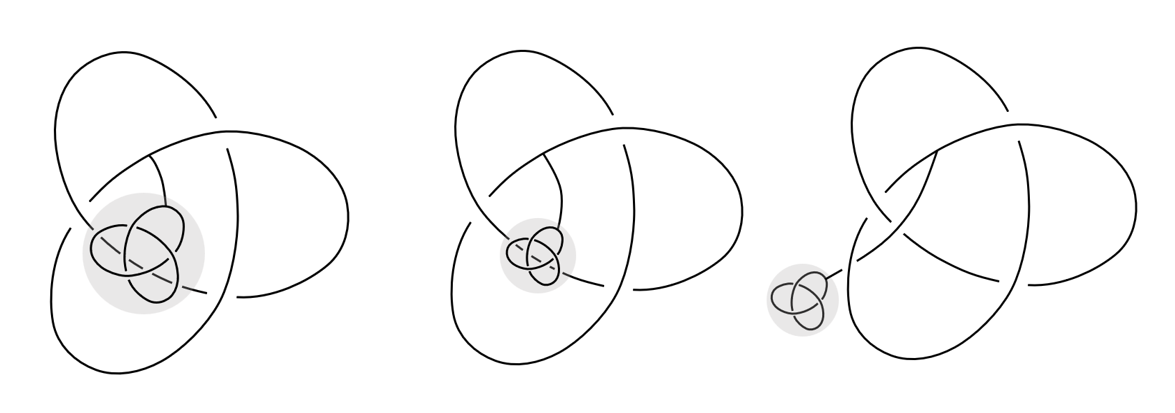
\includegraphics[width=\textwidth]{bouquet_pulling.png}}
    \caption{In a handcuff curve, the process of pulling out the inner bouquet without affecting the rest.}
    \label{figure_1} 
\end{figure*}

\begin{prop}
    For a handcuff curve $H$, let $L$ be a link component of $H$. Then,
    \[ \alpha(H) \geq \alpha(L)+1. \]
\end{prop}
\begin{proof}
    In the arc presentation of $H$, let $v_1$, $v_2$ be the vertices of $H$. Then, there are half-planes that contain the vertex edge of $H$. If we remove them, the remainder is the arc presentation of $L$, the link component of $H$. Since the number of half-planes that contain the vertex edge is at least $1$, we obtain
    \[ \alpha(H) \geq \alpha(L) + (\text{the number of half plane that contain vertex edge}) \geq \alpha(L)+1. \]
\end{proof}

Using the Theorem 1, we obtain the following corollary.

\begin{corol}
    In the handcuff curve $H$, if its link component $L$ is alternating and non-split, then
    \[ \alpha(H) \geq c(L)+3. \]
\end{corol}
\begin{proof}
    Since $L$ is alternating and non-split link, $\alpha(L)=c(L)+2$ by Theorem 1. Thus, \[\alpha(H) \geq \alpha(L)+1 = \left( c(L)+2 \right)+1 = c(L)+3\] according to Proposition 1.
\end{proof}

Combining the above corollary and the corollary of Theorem 2, we have the following theorem.

\begin{theorem}
    For the handcuff curve $H$, if the link component $L$ is alternating and non-split, then
    \[ \alpha(H) = c(L)+3. \]
\end{theorem}

We now consider the Yamada polynomial(주석으로 야마다 달아주고) of the handcuff curve and investigate the relationship between the difference of its maximum and minimum degrees and the arc index.

\begin{defn}
    For a graph $G=(V, E)$, where $V$ is vertex set of $G$ and $E$ is edge set of $G$, let us define $2$-variable Laurent polynomial
    \[ h(G)(x, y) = \sum_{F \subset E} (-x)^{-|F|} x^{\mu(G-F)} y^{\beta(G-F)} \]
    where $\mu(G)$ and $\beta(G)$ is the number of connected components of $G$ and the first Betti number of $G$. \\
    Then, the Yamada polynomial of a graph $G$, $R(G)$ is defined by
    \[ R(G)(x) = h(G)(-1, -x-2-x^{-1}). \]
\end{defn}

It is known that, for some integer $n$, the product $(-x)^n R(G)$ (where $R(G)$ is the Yamada polynomial of the spatial graph $G$) is an ambient isotopy invariant. Moreover, the Yamada polynomial satisfies the following properties.

\begin{theorem}
    For the Yamada polynomial, the following properties hold.
    \begin{enumerate}
        \item $R( \cdot ) = -1$
        \item Let $e$ be a non-loop edge of a graph $G$. Then, $R(G) = R(G / e) + R(G - e)$, where $G/e$, $G-e$ denote the graphs obtained by contracting and deleting the edge $e$, respectively.
        \item Let $e$ be a loop edge of a graph $G$. Then, $R(G) = -(x+1+x^{-1}) R(G-e)$.
        \item Let $G_1 \cup G_2$ be a disjoint union of graphs $G_1$ and $G_2$. Then, $R(G_1 \cup G_2) = R(G_1)R(G_2)$.
        \item Let $G_1 \cdot G_2$ be a union of graphs $G_1$ and $G_2$ having one common point. Then, $R(G_1 \cdot G_2) = -R(G_1)R(G_2)$.
        \item If $G$ has an isthmus, then $R(G)=0$.
    \end{enumerate}
\end{theorem}

\begin{theorem}
    For the Yamada polynomial, the following properties hold.
    \begin{enumerate}
        \item 그림 그려서 넣어야함 각 crossing 부근을 뭐시기뭐시기 한거 그림.
    \end{enumerate}
\end{theorem}

Now, using the stacked tangle representation and the Yamada polynomial, we will prove the following theorem. The following theorem gives a lower bound for the arc index in terms of the Yamada polynomial.

\begin{theorem}
    Let $S_T$ be the closure of stacked tangle of theta curve or handcuff curve. Then,
    \[ \text{spr}(R(S_T)) \leq 2n+2 \]
    where $n$ is the number of crossings in $S_T$ and $\mathrm{spr}(f)$ denotes the spread of $f$, the difference between the maximal and minimal degrees of $f$.
\end{theorem}

\begin{corol}
    If $G$ is a theta curve or handcuff curve, then
    \[ \alpha(G) \geq \frac{5 + \sqrt{4 \mathrm{spr}(R(G)) - 15}}{2}, \]
    except when $G$ is the trivial theta curve.
\end{corol}

\begin{proof}
    Let $S_T$ be the closure of stacked tangle of theta curve or handcuff curve. Let $c_s, c_{ss}, c_n, n$ be the number of simple cap, semi-simple cap, non-simple cap and the number of crossings in $S_T$, respectively. We will prove the theorem using the mathematical induction on the pair $(c_s+c_{ss}, n)$, ordered lexicographically.
    \begin{enumerate}
        \item Basis cases \\
        First, suppose $c_s + c_{ss} = 0$. Then, since there are no simple disks, $S_T$ must be the trivial theta curve. In this case, the number of crossing is at least $1$. Since the spread of Yamada polynomial of trivial theta curve is $4$, $\mathrm{spr}(R(S_T)) = 4 \leq 2n+2$. \\
        Second, suppose $n = 0$. Then, $S_T$ must be the disjoint union of trivial handcuff graph and possibly some circles(unlink). Since the Yamada polynomial of trivial handcuff is zero, $\mathrm{spr}(R(S_T)) = 0 \leq 2 = 2n+2$. \\
        Hence, basis step is proven.
        
        \item Inductive step \\
        Assume that the theorem holds for all pairs $(c_s' + c_{ss}', n') < (c_s + c_{ss}, n)$, and suppose $c_s+c_{ss} > 0$. Then the top disk must have a semi-simple cap. Let the disk connected to the top disk be denoted by $D_s$. (Note that if the top disk had only a non-simple cap, then there would be no simple or semi-simple cap at all.) Since $D_s$ is not top disk, there exists a disk $D$ directly above $D_s$. Now we consider two cases, depending on whether there exists a cap between $D_s$ and $D$. First, suppose that there is no cap between $D_s$ and $D$. Then, there are two possibilities: there is an intersection between $D_s$ and $D$, or there is not. \\
        If there is no intersection between $D_s$ and $D$, we can swap the position of $D_s$ and $D$ without affecting the rest of the diagram. If there is an intersection between $D_s$ and $D$, we can use the relation

        \[ R \left( \Xslashfront \right) - R \left( \Xslashback \right) = (x - x^{-1}) \left( R \left( \czero \right) - R \left ( \cinf \right) \right). \]

        In $S_T$, let $S_T'$, $S_T^0$ and $S_T^\infty$ be the diagrams obtained by replacing the $\Xslashfront$ crossing with $\Xslashback$, $\czero$ and $\cinf$, respectively. Since both $R \left( S_T^0 \right)$ and $R \left ( S_T^\infty \right)$ have $c_s$ simple disks, $c_{ss}$ semi-simple disks, and $n-1$ crossings, their spread is at most $2(n-1)+2=2n$ by the induction hypothesis. Therefore, the spread of $(x - x^{-1}) \left( R \left( S_T^0 \right) - R \left ( S_T^\infty \right) \right)$ is at most $2n+2$. It is thus sufficient to prove that the spread of $R \left ( S_T' \right)$ is at most $2n+2$. Now, observe that $S_T'$ can be interpreted as the diagram obtained by swapping the positions of $D_s$ and $D$ in $S_T$. Therefore, in both cases, it is enough to prove that the inequality holds after this swapping. However, after each swap, the distance between the top disk and $D_s$ decreases. Hence, we can continue swapping $D_s$ with the disk directly above it until either the disk above $D_s$ is the top disk, or there is a cap between $D_s$ and the disk above it. Then it suffices to consider the case where there is a cap between $D_s$ and $D$. \\
        Now, consider the case where there is a cap between $D_s$ and $D$. There are two cases: either $D_s$ is simple or it is non-simple. If $D_s$ is simple, we can reduce the number of caps using Reidemeister moves, as illustrated in Figure 2. Its spread is at most $2n+2$ by the induction hypothesis. Therefore, the spread of $S_T$ is at most $2n+2$. If $D_s$ is non-simple, the number of caps can be similarly reduced using the Reidemeister moves, as shown in Figure 3. \\
    \end{enumerate}
    Hence, by the base cases and the inductive step, the theorem follows by mathematical induction. \\ \\
    Corollary follows by bounding the number of crossings $n$ in terms of the arc index $\alpha(G)$. Suppose $G$ is a theta curve, let $RS_T$ be a reduced stacked tangle with no nested caps. Since the stacked tangle has $2$ non-simple disks and $\alpha(G)-3$ simple disks, the following holds.
    \begin{enumerate}
        \item The number of crossings between simple disks is at most $\binom{\alpha(G)-3}{2}$.
        \item The number of crossings between simple and non-simple disks is at most $2 \cdot (\alpha(G)-3)$.
        \item The number of crossings between the two non-simple disks is at most $2$, except for the trivial theta curve.
    \end{enumerate}
    However, for each cap, the two arcs that it connects have no crossing since $RS_T$ has no nested caps. Moreover, any pair of simple arcs is connected by at most one cap. Note that between the two non-simple disks, there are at most two caps, except in the trivial theta curve case. Therefore, we obtain the following upper bound on $n$ in terms of $\alpha(G)$:
    \[ n \leq \binom{\alpha(G)-3}{2} + 2(\alpha(G)-3) + 2 - (\alpha(G)-2) = \frac{1}{2} (\alpha(G)^2 - 5 \alpha(G) + 8). \]
    Using the above theorem, we have the following inequality:
    \[ \alpha(G) \geq  \frac{5+\sqrt{4\mathrm{spr}(R(G))-15}}{2}. \]
    Now suppose $G$ is a handcuff curve. Similarly, the following holds.
    \begin{enumerate}
        \item The number of crossings between simple disks is at most $\binom{\alpha(G)-3}{2}$.
        \item The number of crossings between simple and non-simple disks is at most $2 \cdot (\alpha(G)-3)$.
        \item The number of crossings between the two non-simple disks is at most $1$.
    \end{enumerate}
    Note that, in contrast to the theta case, some two arcs in a handcuff curve can be connected to two caps simultaneously when a simple arc intersects a non-simple one, because there are two loops in a handcuff curve. Moreover, since a handcuff curve has only one edge connecting the two vertices, there can be at most one cap between the two non-simple disks. Thus, the number of crossings satisfies the same upper bound:
    \[ n \leq \binom{\alpha(G)-3}{2} + 2(\alpha(G)-3) + 1 - (\alpha(G)-1-2) = \frac{1}{2} (\alpha(G)^2 - 5 \alpha(G) + 8), \]
    and we obtain the following inequality:
    \[ \alpha(G) \geq  \frac{5+\sqrt{4\mathrm{spr}(R(G))-15}}{2}. \]
\end{proof}

Figure 2, 3에 각각 푸는 모습 보여줘야함. 아직 더 필요

\begin{theorem}
    뭐시기 출처 모름
\end{theorem}

\section{Research Result}
뭔가 나오긴 하겠지...............?

\section{Conclusion}
요약, 더 나아가서 어떻게 써먹을 수 있을지?

\begin{thebibliography}{9}
    \bibitem{lamport94}
    Leslie Lamport.
    \newblock \LaTeX: A Document Preparation System.
    \newblock Addison Wesley, Reading, Massachusetts, second edition, 1994.
    \bibitem{knuth84}
    Donald E. Knuth.
    \newblock The \TeX book.
    \newblock Addison Wesley, Reading, Massachusetts, 1984.
\end{thebibliography}

\end{document}